\documentclass{beamer}
\usepackage[utf8]{inputenc}

\usepackage{utopia} %font utopia imported
\usepackage{tipa}
\usepackage{ragged2e}
\usetheme{Madrid}
\usecolortheme{default}

%------------------------------------------------------------
%This block of code defines the information to appear in the
%Title page
\title[Git Rebase Workflow] %optional
{Git Rebase Workflow}

\subtitle{Demo Day}


\date[KS 2024] % (optional)
{September 2024}

\logo{
\includegraphics[height=0.8cm]{pictures/prodigy-logo-600x162.png}}

%End of title page configuration block
%------------------------------------------------------------



%------------------------------------------------------------
%The next block of commands puts the table of contents at the 
%beginning of each section and highlights the current section:

\AtBeginSection[]
{
  \begin{frame}
    \frametitle{Table of Contents}
    \tableofcontents[currentsection]
  \end{frame}
}
%------------------------------------------------------------


\begin{document}

%The next statement creates the title page.
\frame{\titlepage}


%---------------------------------------------------------
%This block of code is for the table of contents after
%the title page
\begin{frame}
\frametitle{Table of Contents}
\tableofcontents
\end{frame}
%---------------------------------------------------------

%---------------------------------------------------------
\section{What's a Github?}
\begin{frame}
\frametitle{What's a Github?}
\begin{center}
    
\includegraphics[height=5cm]{pictures/github.jpg}
\end{center}
\end{frame}


\begin{frame}
\frametitle{What's a version control?}
\begin{block}{version control [v\textschwa rZH\textschwa n k\textschwa n'trōl] \textit{noun}}
records changes to a file or set of files and allows you to recall the specific version of the file you want later
\end{block}


    \pause \begin{columns}[T]
    \column{\dimexpr0.5\paperwidth-20pt}
    Pros
    \begin{itemize}
    \item multiple people can work on the same files  
    \item can restore to backup if you made a boo boo
    \item see exactly what was changed, when and by who
    \end{itemize}
    \column{\dimexpr0.5\paperwidth}
    \pause Cons
    \begin{itemize}
    \item Nothing :$\wedge$)
    \pause \item a little bit of a learning curve :$\wedge$(
    \end{itemize}
  \end{columns}

\end{frame}
%---------------------------------------------------------


%---------------------------------------------------------
\section{Merge Workflow}
\begin{frame}
\frametitle{Typical Merge Flow}

  \begin{columns}
    \column{\dimexpr\paperwidth+20pt}
    
\includegraphics[width=\paperwidth]{pictures/merge_flow.png}
  \end{columns}
  \vspace{0.3cm}
    \begin{columns}
    \column{0.33\textwidth}
    Start working on a new feature
    \column{0.36\textwidth}
    Check in your changes to a Git repository
    \column{0.33\textwidth}
    Finish feature and bring changes in to master
  \end{columns}

\end{frame}

\begin{frame}
\frametitle{Typical Merge Flow - Solo Developer}
\begin{columns}
\column{0.5\textwidth}
    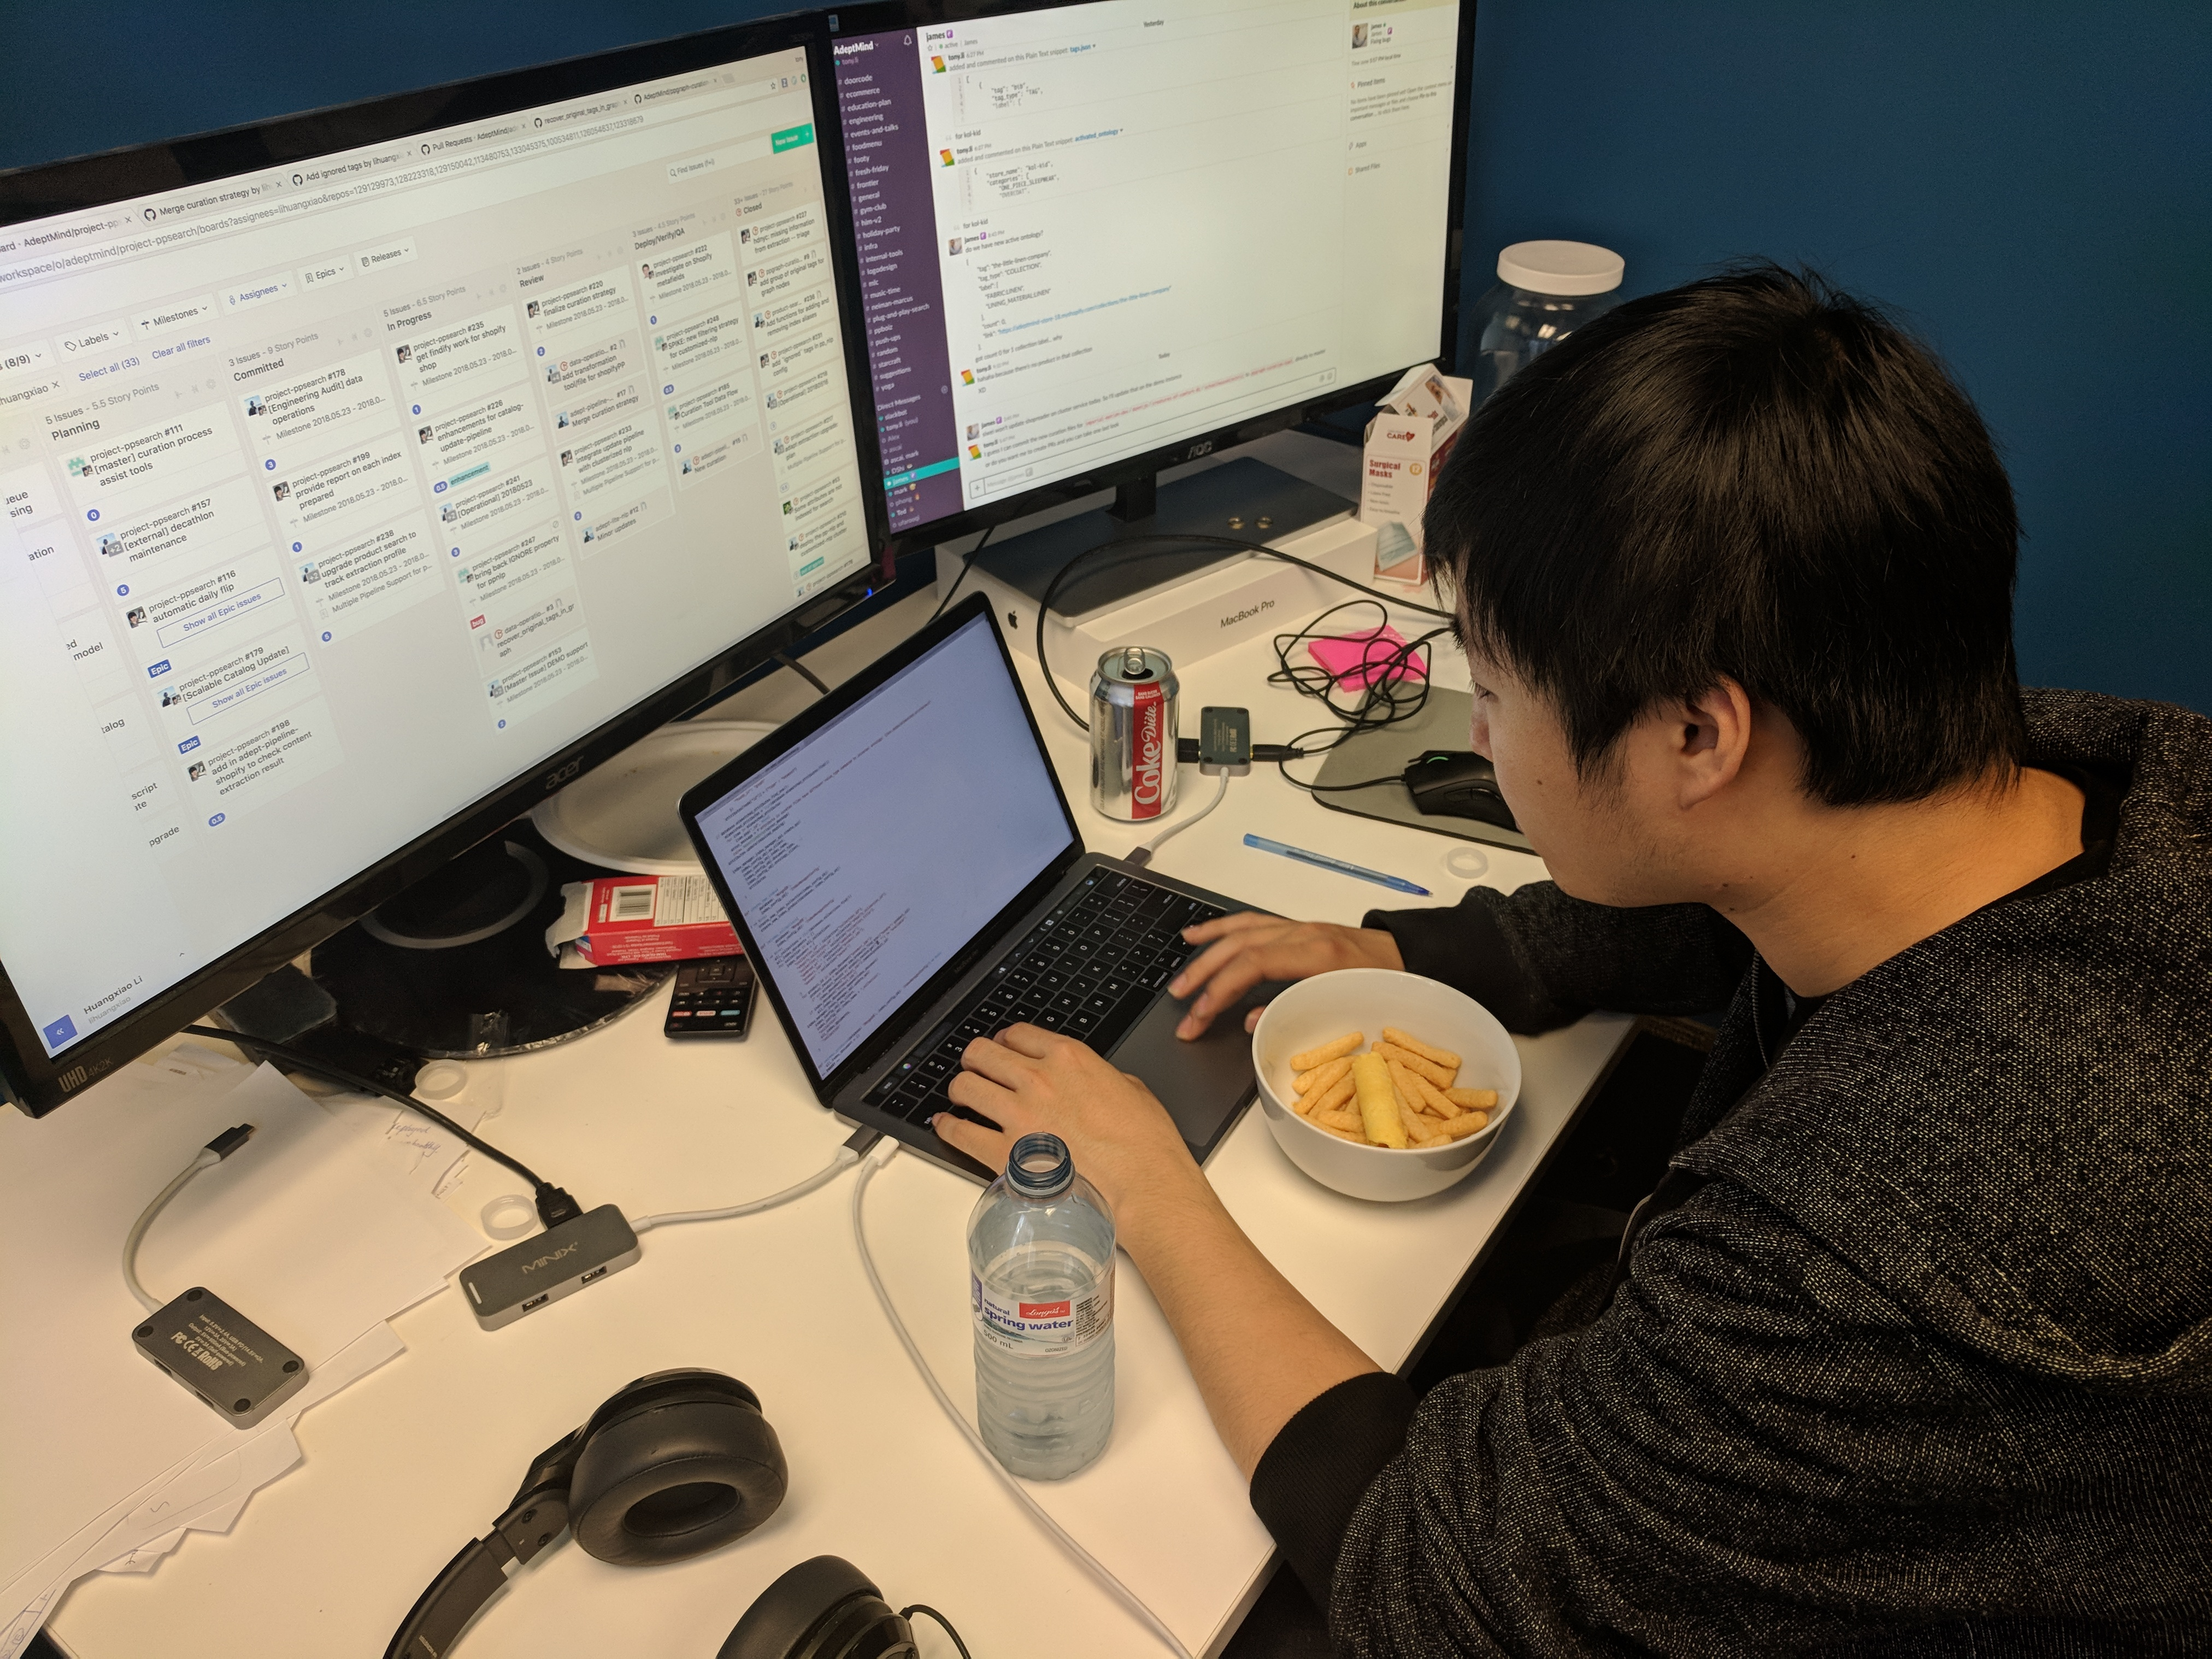
\includegraphics[scale=0.05]{pictures/1_dev.jpg}
\column{0.3\textwidth}
\begin{itemize}
    \item commit directly to master
    \item no conflicts
    \item no wait time for merging
\end{itemize}
\end{columns}
\end{frame}

\begin{frame}
\frametitle{Typical Merge Flow - Solo Developer Git History}
        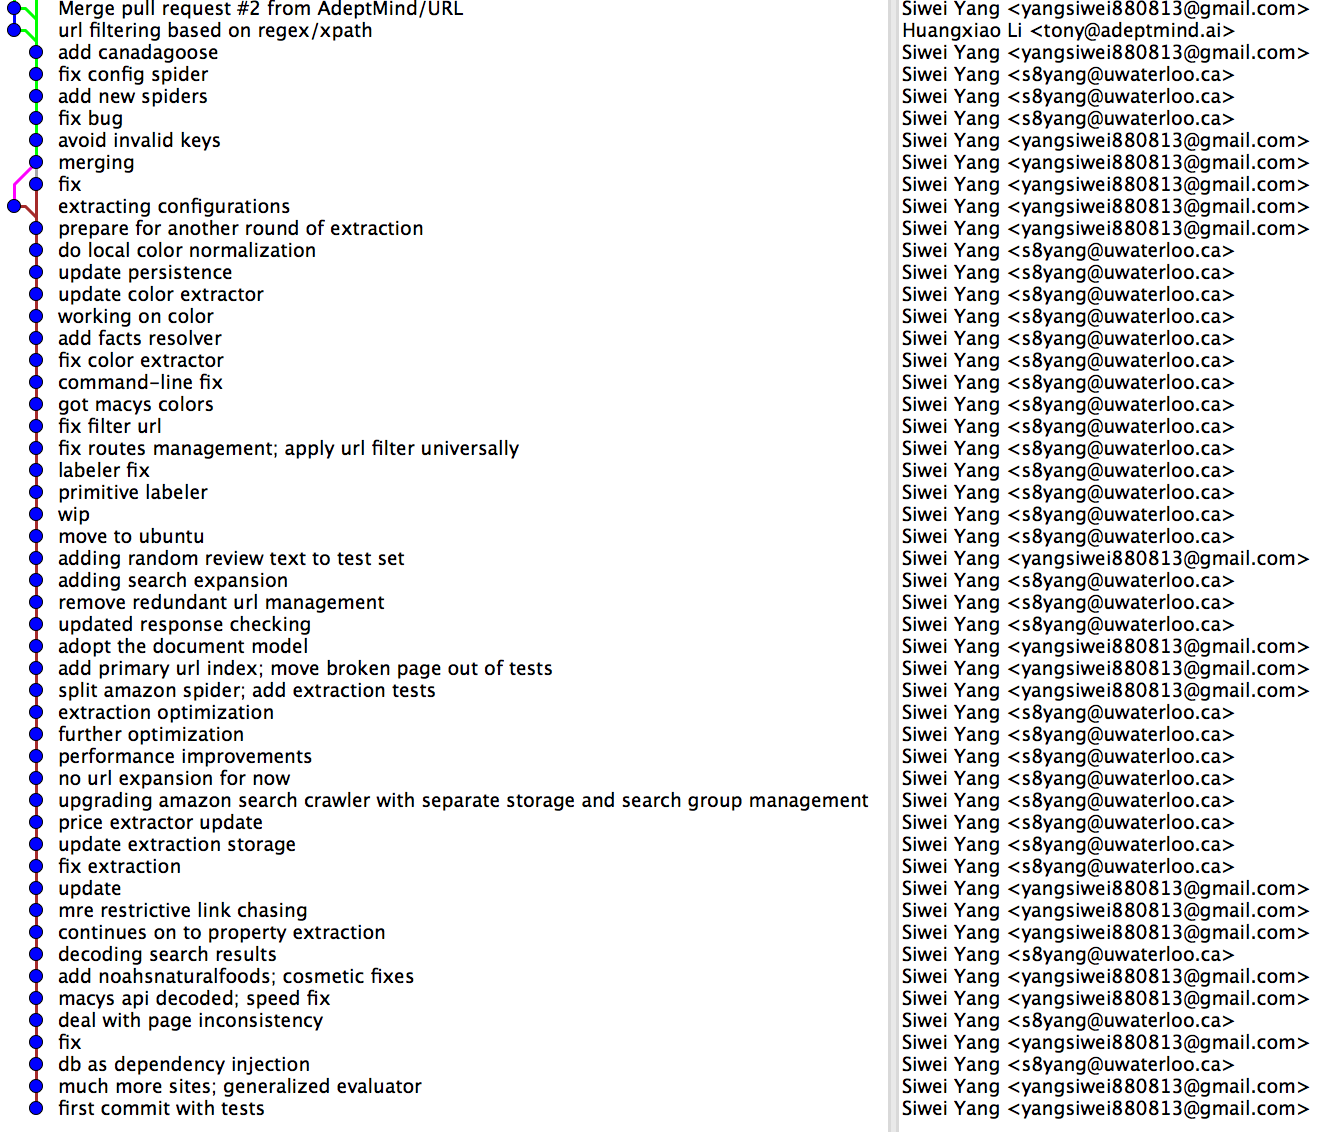
\includegraphics[scale=0.18]{pictures/solo_git.png}
\end{frame}



\begin{frame}
\frametitle{Typical Merge Flow - 2-4 Developers}

\begin{columns}
    \column{0.5\textwidth}
        \includegraphics[scale=0.05]{pictures/2_dev.jpg}
    \column{0.3\textwidth}
        \begin{itemize}
            \item start to use branching strategy
            \item start to see conflicts
            \item need to wait between merges
            \item git history gets more complex, but manageable
        \end{itemize}
\end{columns}
\end{frame}

\begin{frame}
    \frametitle{Typical Merge Flow - 2-4 Developers Git History}
    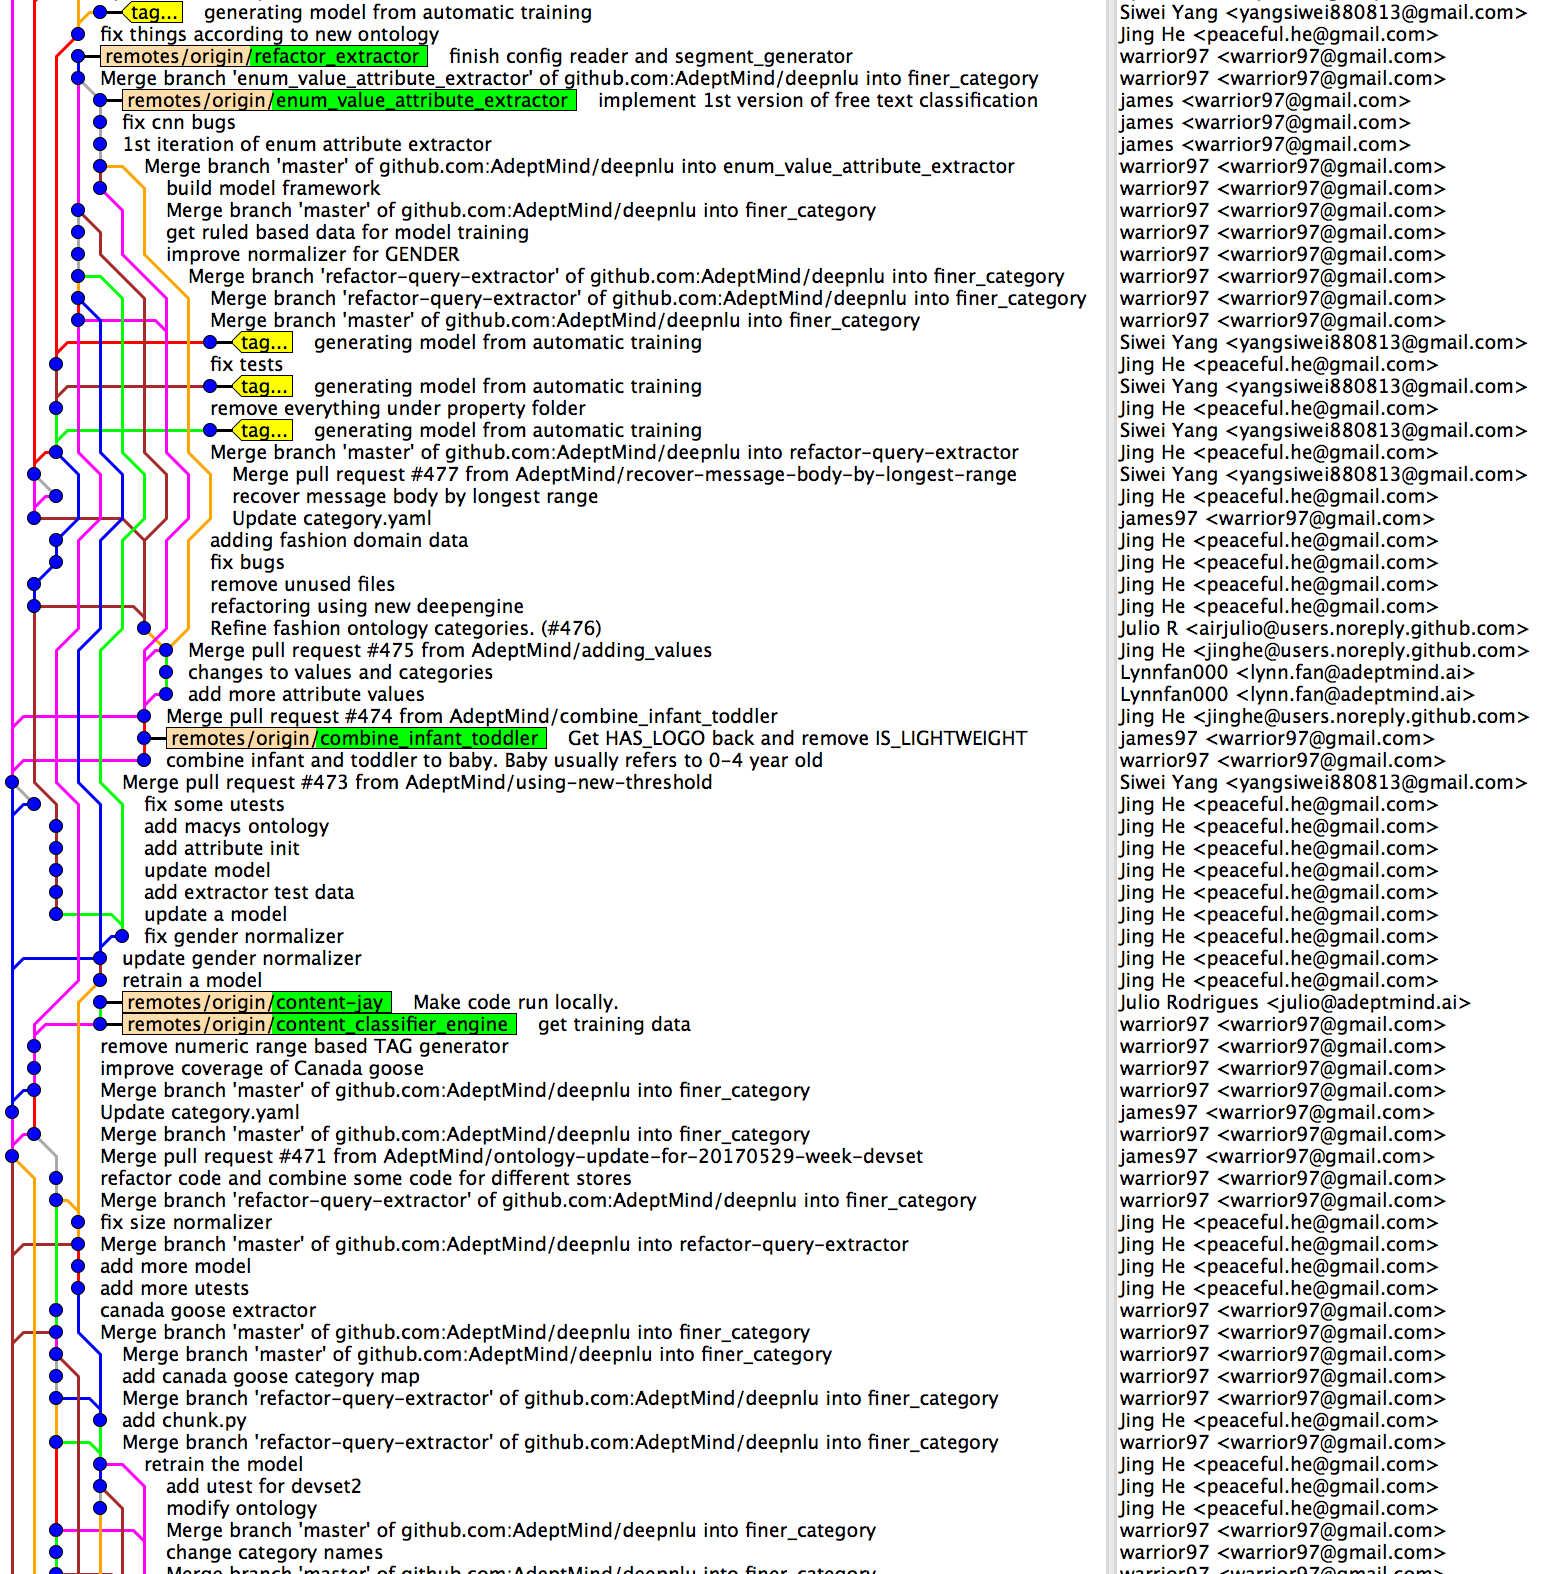
\includegraphics[scale=0.15]{pictures/more_solo_git.png}    
\end{frame}

\begin{frame}
\frametitle{Typical Merge Flow - 5+ Developers}

\begin{columns}
    \column{0.5\textwidth}
        \includegraphics[scale=0.05]{pictures/5_dev.jpg}
    \column{0.3\textwidth}
        \begin{itemize}
            \item lots of branches
            \item start to see conflicts
            \item one developer dedicated to merging
    \end{itemize}
\end{columns}
\end{frame}

\begin{frame}
\frametitle{Typical Merge Flow - 5+ Developers Git History}
    \begin{center}
        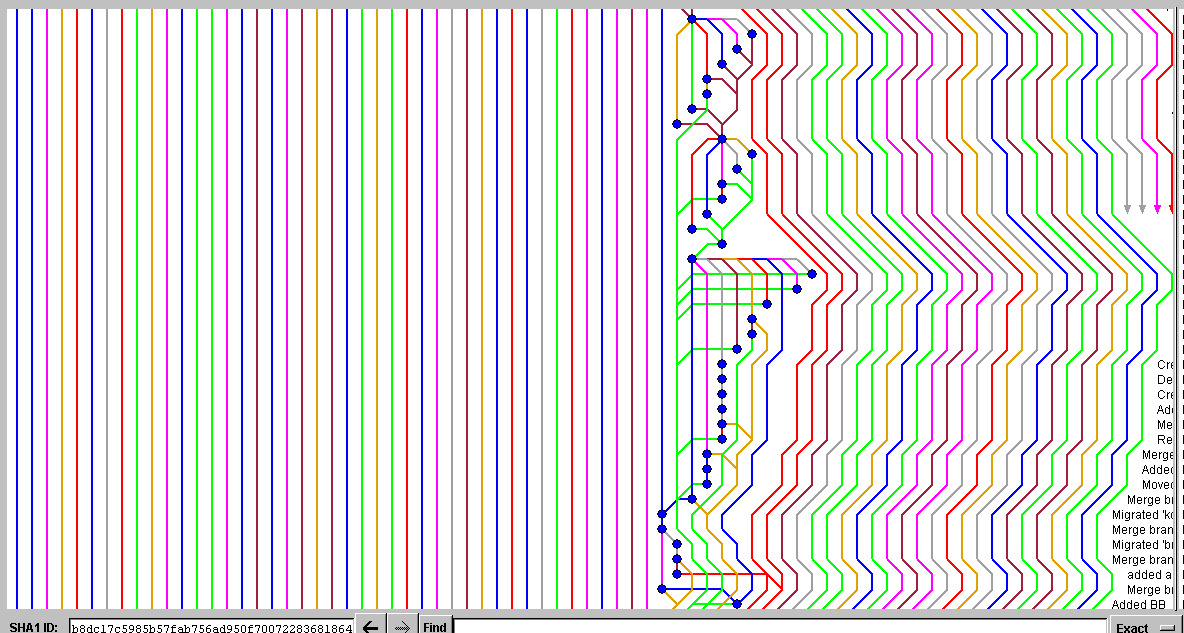
\includegraphics[scale=0.25]{pictures/no.jpg}    
    \end{center}
\end{frame}

\begin{frame}
\frametitle{nonononononononononononononononon stahp STAHP}
    \begin{center}
        
\includegraphics[scale=1.4]{pictures/thisisfine.jpg}    
    \end{center}
\end{frame}

%---------------------------------------------------------


%---------------------------------------------------------
\section{Rebase Workflow}
\begin{frame}
\frametitle{What do?}
\begin{block}{Solution}
    \begin{itemize}
        \item \texttt{git pull --rebase origin master}
        \item \texttt{git rebase -i origin/master}  
    \end{itemize}
\end{block}

\pause \begin{itemize}
    \item Creates a linear history
    \item Easy to handle product release, backporting and release
    \item Conflicts are solved by one developer, and everyone else gets resolutions for free (mostly)
    \item Proven to scale, as proven by all large open source projects
\end{itemize}
\end{frame}

\begin{frame}
\frametitle{Rebase Flow - Taste the Teamwork}
\begin{center}
  \begin{columns}
    \column{\dimexpr\paperwidth+20pt}
    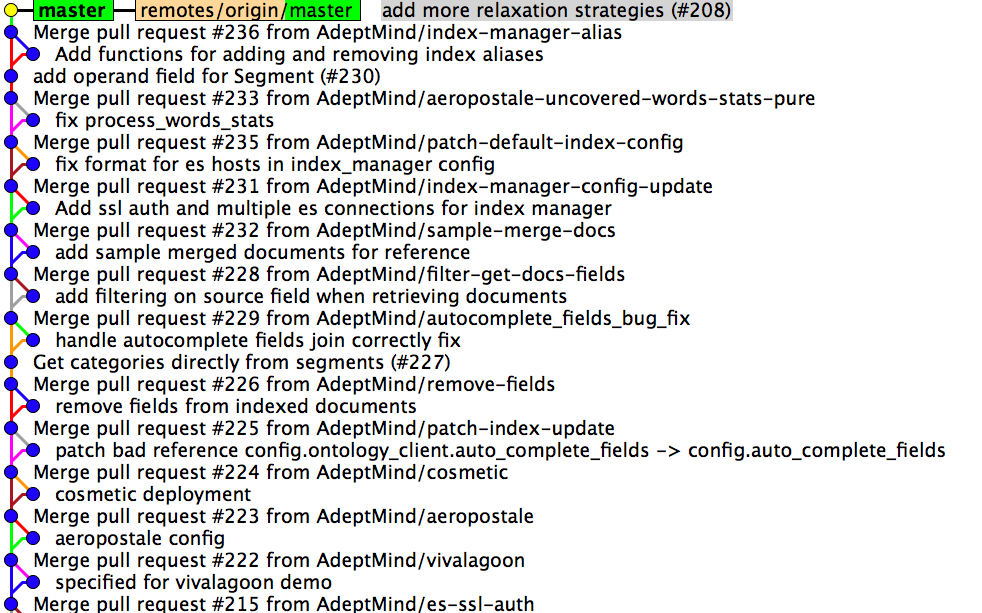
\includegraphics[width=\paperwidth]{pictures/nice.png}
    \end{columns}
\end{center}
\end{frame}

\begin{frame}
\frametitle{What's the Difference, Actually?}
\begin{center}
  \begin{columns}
    \column{\dimexpr\paperwidth+20pt}
    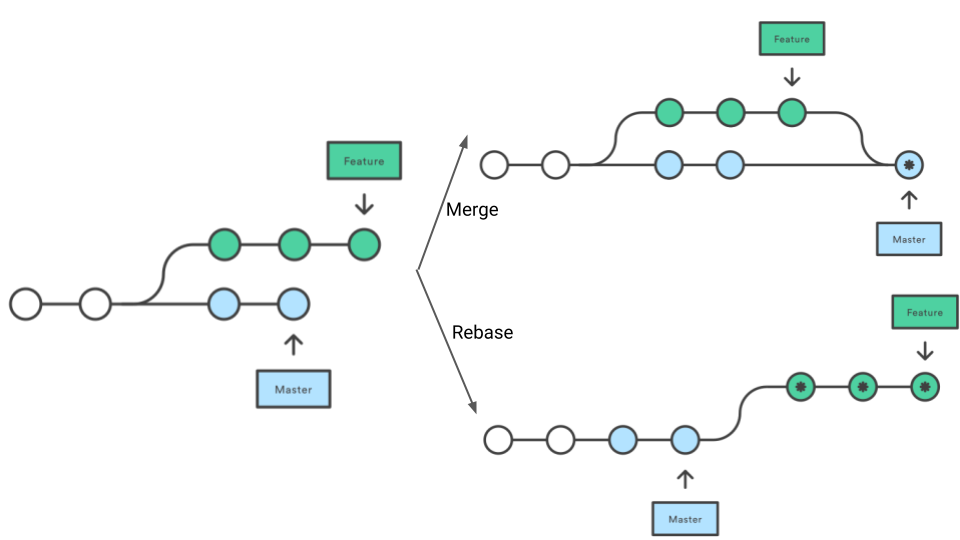
\includegraphics[width=\paperwidth]{pictures/merge_or_rebase.png}
    \end{columns}
\end{center}
\end{frame}

\begin{frame}
\frametitle{Rebase Flow}
\begin{center}
  \begin{columns}[c]
    \column{\dimexpr\paperwidth+20pt}
    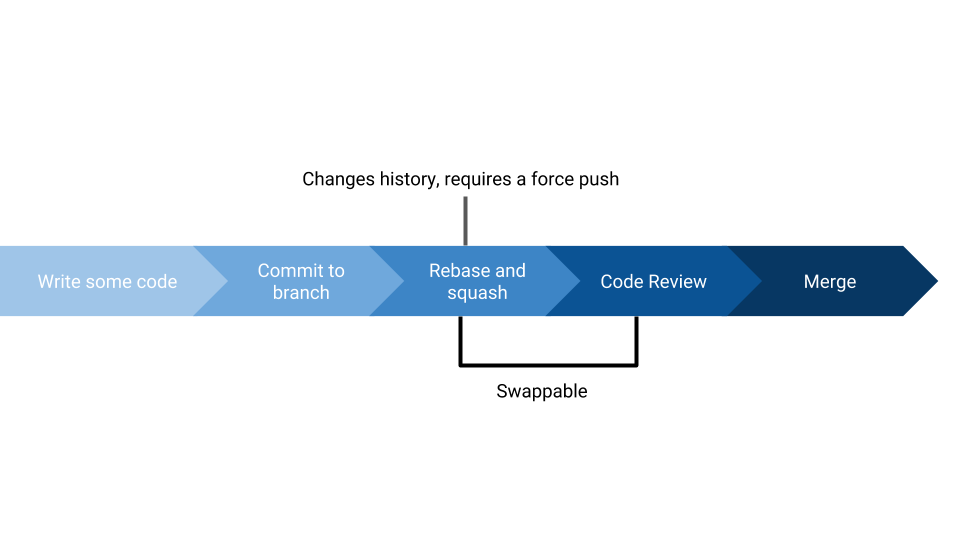
\includegraphics[width=\paperwidth]{pictures/rebase_workflow.png}
    \end{columns}
\end{center}
\end{frame}

\begin{frame}
\frametitle{Only You Can Prevent Forest Fires}
\begin{center}
    
\includegraphics[scale=0.2]{pictures/destruction.jpg}
\end{center}
\end{frame}
%---------------------------------------------------------

\section{Pre-Demo Warmup}


\begin{frame}
\frametitle{Recap Git Fundamentals}
\begin{block}{what am I doing?}
    \begin{itemize}
        \item \texttt{git branch}
        \item \texttt{git status}
        \item \texttt{git diff}
        \item \texttt{gitk --all}
    \end{itemize}
\end{block}

\begin{block}{making changes}
    \begin{itemize}
        \item \texttt{git checkout}
        \item \texttt{git commit}
        \item \texttt{git push}
    \end{itemize}
\end{block}

\begin{block}{rewriting history}
    \begin{itemize}
        \item \texttt{git pull --rebase}
        \item \texttt{git rebase -i}
        \item \texttt{git remote prune origin}
    \end{itemize}
\end{block}

\end{frame}

\begin{frame}
\frametitle{TEAM?!}
\begin{center}
    {\Huge Thank you}

    (demo time?)
\end{center} 
\end{frame}


\end{document}
